\chapter{System}
\section{Einleitung}
Dieses Kapitel bietet eine grobe Übersicht über das ganze System, um die Zusammenhänge zwischen einzelnen Komponenten aufzuzeigen.
Auf einzelne Komponenten wird in folgenden Kapitel genauer eingegangen.

\section{Schematische Übersicht}
In der Abbildung \ref{fig:UebersichtDebuggerToolchain} ist das ganze System abgebildet.
Auf dem \textit{Windows PC} wird die Deep Applikation in Eclipse geschrieben, kompiliert und debuggt.
Plug-Ins erweitern Eclipse um die notwendige Funktionalitäten, die für die Entwicklung von Deep Applikationen notwendig sind.
Es sind beide Debug Toolchains, die ''klassische'' Abatron Toolchain und die neue OpenOCD Toolchain in dieser Übersicht abgebildet.

Bei der Abatron Toolchain wird das Abatron BDI 3000 über die rote TCP/IP Verbindung angesprochen.
Das BDI kommuniziert dann über eine JTAG Verbindung direkt mit dem Zynq Chip.

Die grünen Pfeile zeigen den Kommunikationsweg für die neuen OpenOCD-Toolchains.
OpenOCD bildet zusammen mit der richtigen Hardware, hier ist es der FT2232 Chip, einen kompletten Debugger und ist somit eine Alternative zum BDI.
OpenOCD stellt einen GDB Server und auch ein \textit{Command Line Interface} (CLI) zur Verfügung.
% referenz zu openOCDInterface
Das Eclipse Plugin \textit{openOCDInterface} verwendet das CLI über den TCP/IP Port 4444 (dunkelgrüner Pfeil).
Der GDB Client kommuniziert mit dem GDB Server mit dem GDB Protokoll über den TCP/IP Port 3333 (hellgrüner Pfeil).
OpenOCD verwendet dann den \textit{WinUSB} Treiber um mit dem FT2232 Chip zu kommunizieren.
Der FT2232 verwendet den selben JTAG Bus wie das BDI 3000 als Verbindung mit dem Zynq.

Das \textit{Zybo} beinhaltet neben dem FT2232 auch noch diverse I/O Peripherie die in einer Deep Applikation genutzt werden kann.
Der FT2232 Chip übernimmt zwei verschiedene Funktionen.
Zum einen wird er als USB zu UART Brücke verwendet, damit man mit dem Windows PC einfach eine serielle Verbindung mit dem Prozessor aufbauen kann.
Zusätzlich fungiert er ebenfalls als Brücke zum JTAG Bus.
Das bedeutet, er erhält Befehle von OpenOCD über USB und übersetzt diese elektrisch und auch logisch für das JTAG Interface.

\begin{figure}[htbp]
	\centering
		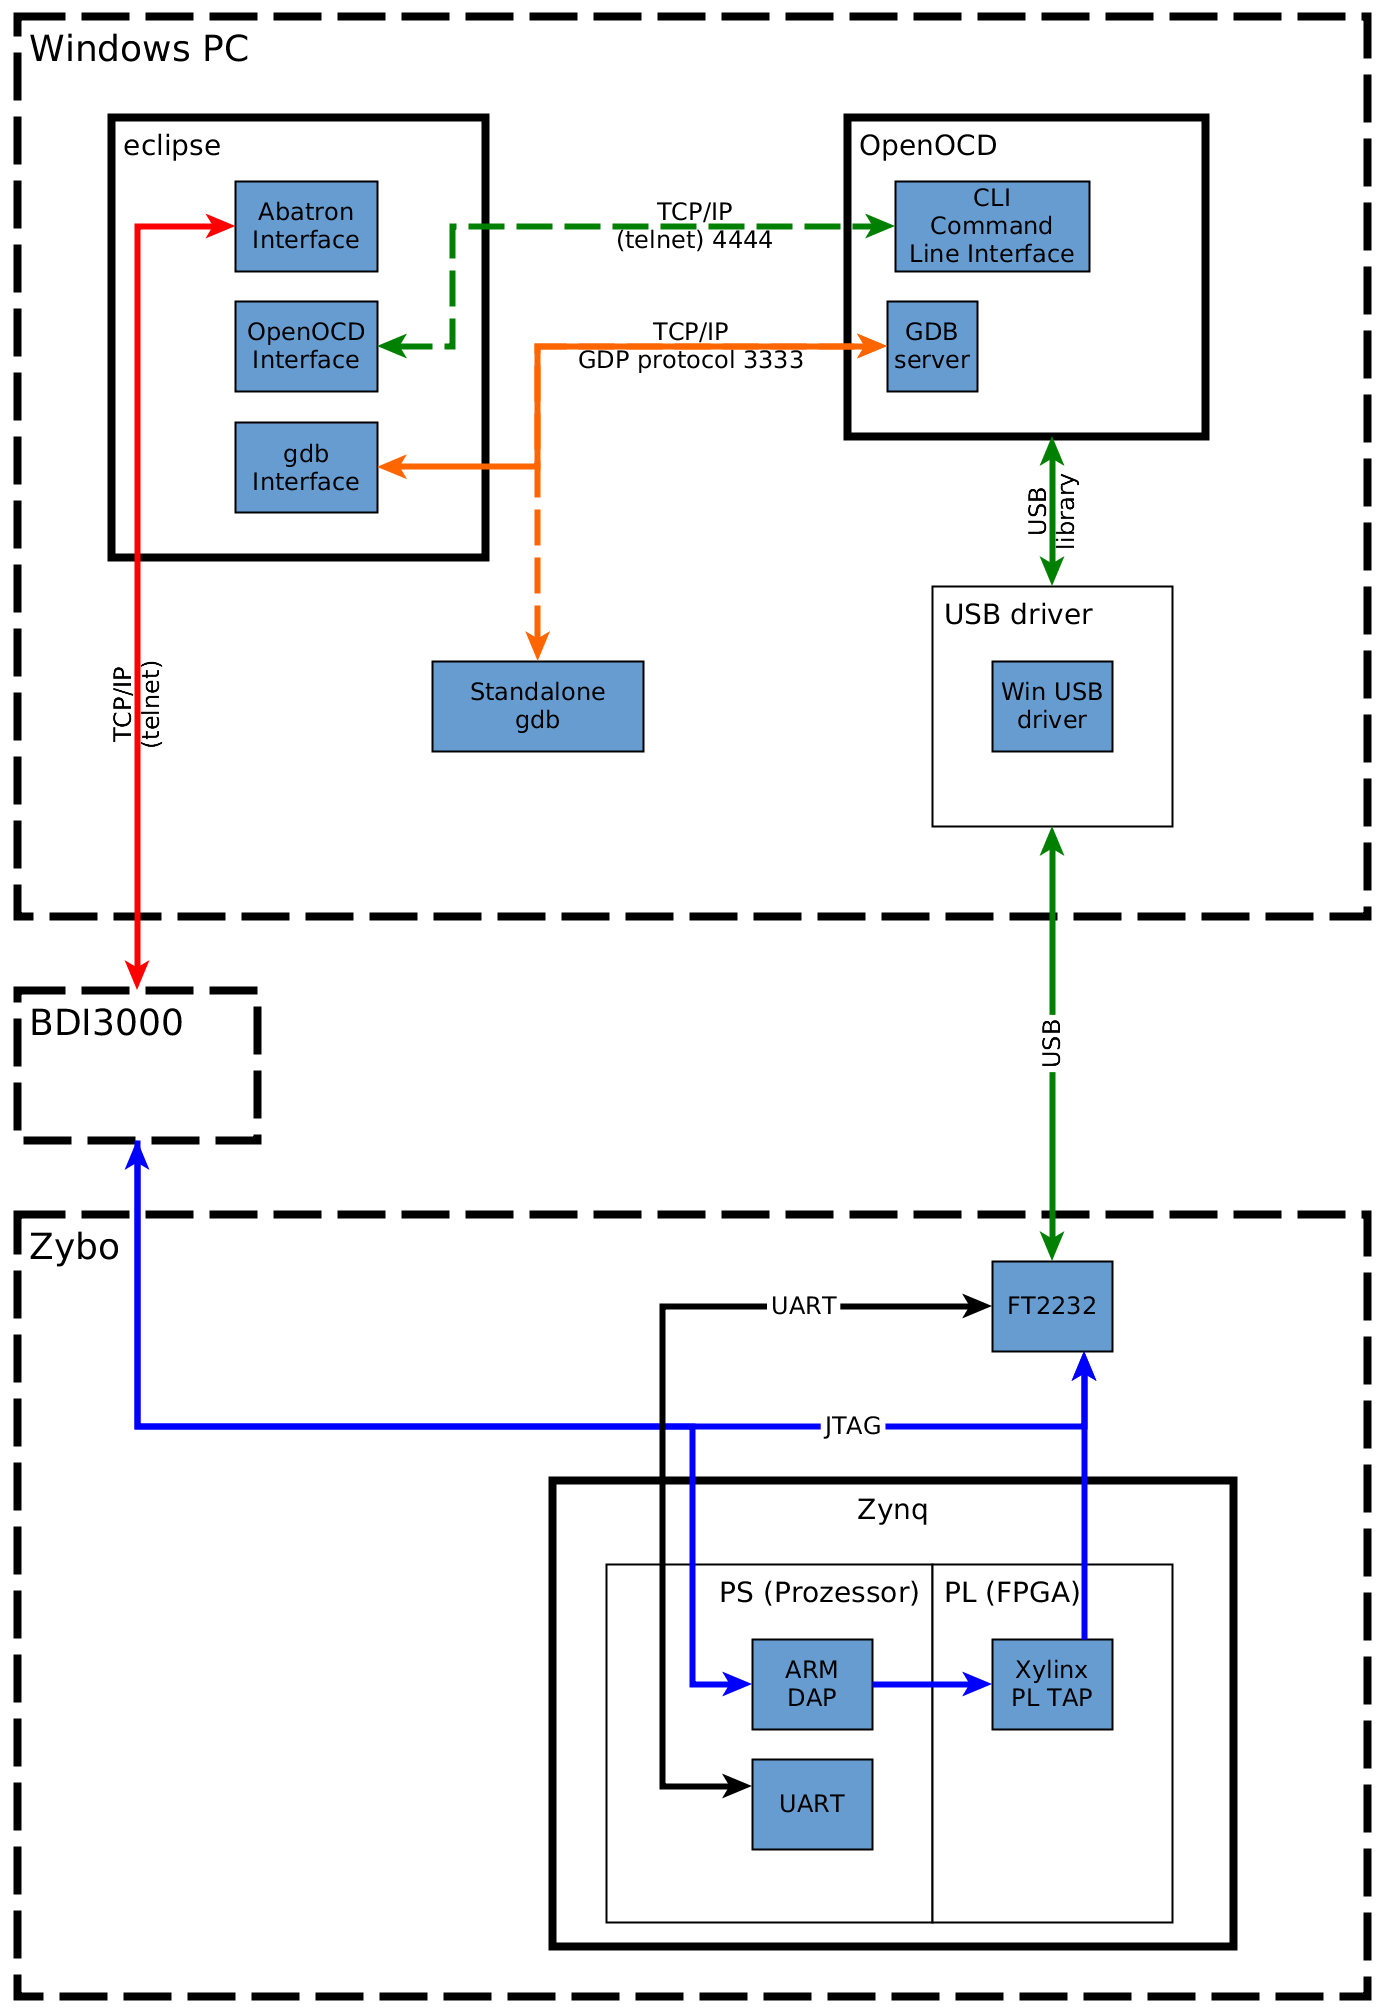
\includegraphics[width=\textwidth,height=\textheight,keepaspectratio]{graphs/embeddedDebuggerToolchain.png}
	\caption{Systemübersicht Debugger Toolchain}
	\label{fig:UebersichtDebuggerToolchain}
\end{figure}


\section{Debugger Toolchains}
\subsection{Abatron-Toolchain}
Die Abatron-Toolchain benötigt weder OpenOCD noch den FT2232, dafür aber das teure BDI 3000.
Diese ''klassische'' Toolchain wird für die Entwicklung von Deep Applikationen für den PowerPC verwendet.
In dieser Arbeit wird sie aber nicht direkt verwendet.


\subsection{CLI-OpenOCD-Toolchain}
Das teure BDI wird für diese Toolchain nicht mehr benötigt.
% verbessern: satzbau
Da das CLI\footnote{Command Line Interface} von OpenOCD ist aber sehr ähnlich wie das CLI des BDI.
% Es nutzt ebenfalls das Telnet Protokoll.
Eine Portierung ist somit relativ einfach.
Die CLI-OpenOCD-Toolchain lehnt sich deshalb sehr stark an die bestehende Abatron Toolchain an.
% Die bestehende Toolchain für den PPC ist nicht auf der offiziellen Deep Homepage dokumentiert.

Mit dieser Toolchain ist \textit{Source Code Debugging} aber nicht möglich.
Das bedeutet, es ist nicht möglich im Source Code Breakpoints zu setzten, oder durch einzelne Zeilen im Source Code zu steppen wie man es von Debuggern wie dem GDB gewohnt ist.
% TODO wirklich target commands?
Bestehende Möglichkeiten aus der alten Abatron-Toolchain wie \textit{Target Commands} bleiben aber erhalten.


\subsection{GDB-OpenOCD-Toolchain}
In der GDB-OpenOCD-Toolchain wird, wie bei der obigen Toolchain, ebenfalls die OpenOCD Software und der FT2232 Chip verwendet.
Es wird aber nicht mehr ein Interface bestehend auf der ''klassischen'' Abatron Toolchain verwendet, sondern es wird direkt der bekannte GDB in Eclipse verwendet.
Dadurch kann \textit{Source Code Debugging} direkt in Eclipse eingesetzt werden.
% für unterricht
% in line debugging
% günstige hardware

